% !TeX spellcheck = en_US
%%%%%%%%%%%%%%%%%%%%%%%%%%%%%%%%%%%%%%%%%%%%%%%%%%%%%%%%%%%%%%%%%%%%%%%%%%%%%%%%
%2345678901234567890123456789012345678901234567890123456789012345678901234567890
%        1         2         3         4         5         6         7         8

\documentclass[letterpaper, 10 pt, conference]{ieeeconf}  % Comment this line out if you need a4paper

%\documentclass[a4paper, 10pt, conference]{ieeeconf}      % Use this line for a4 paper

\IEEEoverridecommandlockouts                              % This command is only needed if 
                                                          % you want to use the \thanks command

\overrideIEEEmargins                                      % Needed to meet printer requirements.

% See the \addtolength command later in the file to balance the column lengths
% on the last page of the document

% The following packages can be found on http:\\www.ctan.org
%\usepackage{graphics} % for pdf, bitmapped graphics files
%\usepackage{epsfig} % for postscript graphics files
%\usepackage{mathptmx} % assumes new font selection scheme installed
%\usepackage{times} % assumes new font selection scheme installed
\usepackage{float}
\usepackage{ngerman}
\usepackage[utf8]{inputenc}
\usepackage{color}
\usepackage{amsmath}
\usepackage{bm}
\usepackage{amssymb}
\usepackage{graphicx}
\graphicspath{{./figures/}}
% Symbole für Tabelle: grüner Haken und rotes Kreuz
\newcommand{\ok}{{\color{green}\checkmark}}
\newcommand{\no}{{\color{red}$\boldsymbol\times$}}

\usepackage{calrsfs}
\DeclareMathAlphabet{\pazocal}{OMS}{zplm}{m}{n}
\newcommand{\body}[1]{\mathcal{B}_{#1}}
\newcommand{\ks}[1]{\mathcal{F}_{#1}}
\newcommand{\cc}[1]{\mathcal{C}_{#1}}
\newcommand{\ortvek}[3]{{ }_{(#1)}{\boldsymbol{r}}^{#2}_{#3}}

% Geometrische Bezeichnungen des Mechanismus. Sind in schriftlichen Aufzeichnungen nicht konsistent. Daher wird die Benennung in diesem Paper geändert. Zur Übersichtlichkeit werden die alten Bezeichnungen als Makro verwendet.
% https://tex.stackexchange.com/a/9728
\makeatletter
\newcommand{\gdelta}{\afterassignment\gdelta@aux\count0=}
\newcommand{\gdelta@aux}{\csname gdelta\the\count0\endcsname}
\newcommand{\gdotdelta}{\afterassignment\gdotdelta@aux\count0=}
\newcommand{\gdotdelta@aux}{\csname gdotdelta\the\count0\endcsname}
\newcommand{\ggamma}{\afterassignment\ggamma@aux\count0=}
\newcommand{\ggamma@aux}{\csname ggamma\the\count0\endcsname}
\newcommand{\gbeta}{\afterassignment\gbeta@aux\count0=}
\newcommand{\gbeta@aux}{\csname gbeta\the\count0\endcsname}
\newcommand{\gl}{\afterassignment\gl@aux\count0=}
\newcommand{\gl@aux}{\csname gl\the\count0\endcsname}
\newcommand{\ghl}{\afterassignment\ghl@aux\count0=}
\newcommand{\ghl@aux}{\csname ghl\the\count0\endcsname}
\makeatother

\newif\ifneuenomenklatur
\neuenomenklaturtrue

% Neue Bezeichnungen:
\ifneuenomenklatur
    \expandafter\newcommand\csname gdelta8\endcsname{%
        \eta_1}
    \expandafter\newcommand\csname gdelta6\endcsname{%
        \eta_2}
    \expandafter\newcommand\csname gdelta16\endcsname{%
        \eta_3}
    \expandafter\newcommand\csname gdelta3\endcsname{%
        \eta_4}
    \expandafter\newcommand\csname gdelta19\endcsname{%
        \eta_5}
    \expandafter\newcommand\csname gdotdelta19\endcsname{%
        \dot{\eta}_5}
    \expandafter\newcommand\csname gdelta17\endcsname{%
        \eta_6}
    \expandafter\newcommand\csname gbeta1\endcsname{%
        \eta_7}
    \expandafter\newcommand\csname gdelta18\endcsname{%
        \eta_8}
    \expandafter\newcommand\csname ggamma5\endcsname{%
        \eta_9}
    \expandafter\newcommand\csname ggamma3\endcsname{%
        \eta_{10}}
    \expandafter\newcommand\csname gdelta7\endcsname{%
        \eta_{11}}
    \expandafter\newcommand\csname gl1\endcsname{%
        L_1}
    \expandafter\newcommand\csname gl2\endcsname{%
        L_2}
    \expandafter\newcommand\csname gl3\endcsname{%
        L_3}
    \expandafter\newcommand\csname gl4\endcsname{%
        L_8}
    \expandafter\newcommand\csname gl5\endcsname{%
        L_4}
    \expandafter\newcommand\csname gl6\endcsname{%
        L_9}
    \expandafter\newcommand\csname gl11\endcsname{%
        2L_5}
    \expandafter\newcommand\csname ghl11\endcsname{%
        L_5}
    \expandafter\newcommand\csname gl12\endcsname{%
        2L_6}
    \expandafter\newcommand\csname ghl12\endcsname{%
        L_6}
    \expandafter\newcommand\csname gl13\endcsname{%
        L_{13}}
    \expandafter\newcommand\csname gl14\endcsname{%
        L_{11}}
    \expandafter\newcommand\csname gl15\endcsname{%
        L_7}
    \expandafter\newcommand\csname gl20\endcsname{%
        L_{12}}
    \expandafter\newcommand\csname gl22\endcsname{%
        L_{10}}
    \expandafter\newcommand\csname gl16\endcsname{%
        L_\mathrm{spring}}
\else
    % Original-Bezeichnungen:
    \expandafter\newcommand\csname gdelta8\endcsname{%
        \delta_8}
    \expandafter\newcommand\csname gdelta6\endcsname{%
        \delta_6}
    \expandafter\newcommand\csname gdelta16\endcsname{%
        \delta_{16}}
    \expandafter\newcommand\csname gdelta3\endcsname{%
        \delta_3}
    \expandafter\newcommand\csname gdelta19\endcsname{%
        \delta_{19}}
    \expandafter\newcommand\csname gdotdelta19\endcsname{%
        \dot{\delta}_{19}}
    \expandafter\newcommand\csname gdelta17\endcsname{%
        \delta_{17}}
    \expandafter\newcommand\csname gbeta1\endcsname{%
        \beta_1}
    \expandafter\newcommand\csname gdelta18\endcsname{%
        \delta_{18}}
    \expandafter\newcommand\csname ggamma5\endcsname{%
        \gamma_5}
    \expandafter\newcommand\csname ggamma3\endcsname{%
        \gamma_3}
    \expandafter\newcommand\csname gdelta7\endcsname{%
        \delta_7}
    \expandafter\newcommand\csname gl1\endcsname{%
        l_1}
    \expandafter\newcommand\csname gl2\endcsname{%
        l_2}
    \expandafter\newcommand\csname gl3\endcsname{%
        l_3}
    \expandafter\newcommand\csname gl4\endcsname{%
        l_4}
    \expandafter\newcommand\csname gl5\endcsname{%
        l_5}
    \expandafter\newcommand\csname gl6\endcsname{%
        l_6}
    \expandafter\newcommand\csname gl11\endcsname{%
        l_{11}}
    \expandafter\newcommand\csname ghl11\endcsname{%
        l_{11}/2}
    \expandafter\newcommand\csname gl12\endcsname{%
        l_{12}}
    \expandafter\newcommand\csname ghl12\endcsname{%
        l_{12}/2}
    \expandafter\newcommand\csname gl13\endcsname{%
        l_{12}}
    \expandafter\newcommand\csname gl14\endcsname{%
        l_{14}}
    \expandafter\newcommand\csname gl15\endcsname{%
        l_{15}}
    \expandafter\newcommand\csname gl20\endcsname{%
        l_{20}}
    \expandafter\newcommand\csname gl22\endcsname{%
        l_{22}}
    \expandafter\newcommand\csname gl16\endcsname{%
        l_\mathrm{F}}
\fi

\title{\LARGE \bf
Kinematics and Dynamics Model via Explicit Trigonometric Elimination of Kinematic Constraints for a Force Assistance Exoskeleton
}


\author{Moritz Schappler$^{1}$ and Sami Haddadin$^{2}$% <-this % stops a space
\thanks{*This work was supported by the German Federal Ministry of Education and Research (BMBF) under Grant no. 16SV6175}% <-this % stops a space
\thanks{$^{1}$Moritz Schappler
        {\tt\small moritz.schappler@imes.uni-hannover.de}}%
\thanks{$^{2}$Sami Haddadin
        {\tt\small haddadin@irt.uni-hannover.de}}%
}


\begin{document}



\maketitle
\thispagestyle{empty}
\pagestyle{empty}


%%%%%%%%%%%%%%%%%%%%%%%%%%%%%%%%%%%%%%%%%%%%%%%%%%%%%%%%%%%%%%%%%%%%%%%%%%%%%%%%
\begin{abstract}
abstract

\end{abstract}


%%%%%%%%%%%%%%%%%%%%%%%%%%%%%%%%%%%%%%%%%%%%%%%%%%%%%%%%%%%%%%%%%%%%%%%%%%%%%%%%
\section{Introduction and State of the Art}

Exoskeletons for assistance and rehabilitation

list different upper limb exoskeletons with different concepts

techniques and tools for kinematics and dynamics modeling

model assumptions for wearable robots: kinematic coupling of human and exoskeleton. Exoskeleton may contain passive joints (unlike serial chain robots), floating base assumption for base forces

contributions of the paper:
presentation of a novel exoskeleton mechanism designed
explicit kinematics and dynamics modeling for hybrid mechanism with gear and closed loop kinematic constraints
new approach for implementation of kinematic constraints in explicit form optimized for processing with computer algebra systems.

paper structured as follows: scenario and system presentation, detailed kinematics and dynamics model, control concepts for the system, simulation environment and simulation results.

\section{Exoskeleton and Scenario}

\subsection{Scenario}

force assistance for craftsmen
project goals \cite{NuelleSchTapLil2017}: 
* reduce fatigue of the worker and work-induced diseases, 
* increase work quality by projection of additional information (augmented reality, \cite{NuelleBriTapDem2018})
* guiding the user

This continues the work presented in \cite{PetereitAlbJerSch2012}. 
The waist-carried demonstrator was tested under aspects of ergonomics and workspace and failed. Thus a concept of upper limb exoskeletons proximal to the users body were developed.

\subsection{Exoskeleton}

The exoskeleton consists of several parts which will be introduced in short before being studied closer regarding kinematics and dynamics models.

\subsubsection{Main structure following the Human Arm}

With the attachment at the users upper body and at the hand of the user given with the constraint of neither blocking the users workspace nor sight, the main structure of the exoskeleton follows the arm of the user closely with similar degrees of freedom.

Fig.\,\ref{fig:KAS5_CAD} shows a CAD model of the complete exoskeleton to be carried in a right-hand configuration.


\begin{figure}[tb!]
    \input{./figures/KAS5_Seitenansicht_beschriftet.pdf_tex}
    \caption{CAD model of the exoskeleton mechanism.}
    \label{fig:KAS5_CAD}
\end{figure} 

\subsubsection{Three-Axis Elbow Joint}

The elbow joint of the mechanism is supposed to be on the axis of rotation of the users elbow.
To avoid constraint forces on the users elbow, the joint consists of three parallel axes which couple the upper arm and the forearm via a central gear wheel. The mechanism is shown in detail in Fig.\,\ref{fig:EllenbogenSimMech} with different poses.
The lever mechanism connecting the linear spring-damper-system with the elbow is fixed to the central elbow gear.

\begin{figure}[tb!]
    \begin{tabular}{c c c}
        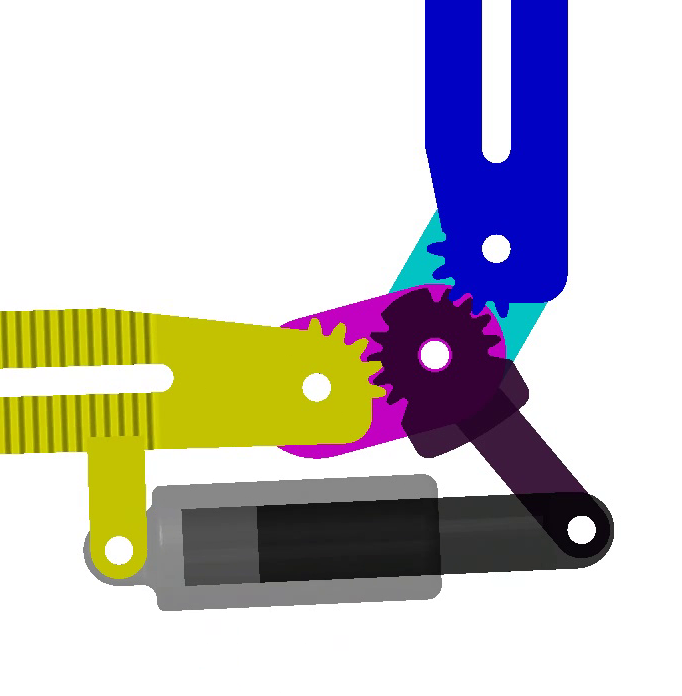
\includegraphics[height=0.5\linewidth]{figures/KAS6m3_SimMech_2.png} &
        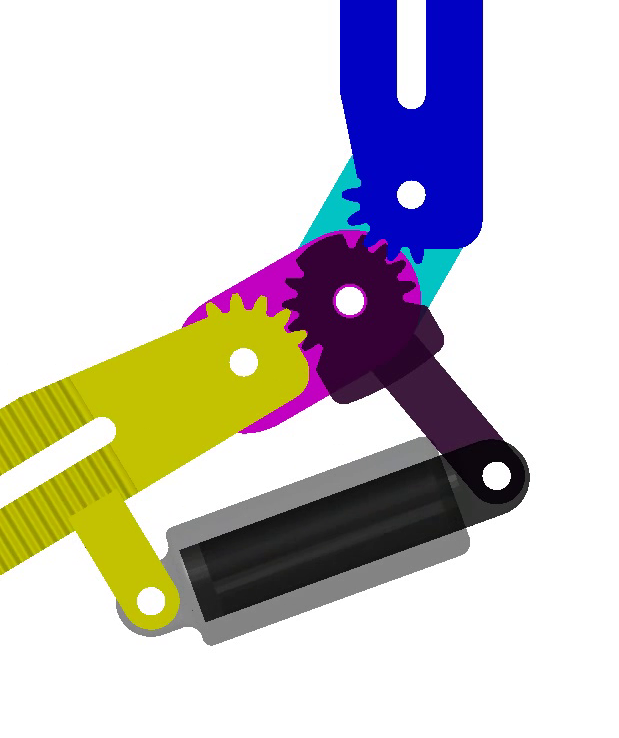
\includegraphics[height=0.5\linewidth]{figures/KAS6m3_SimMech_3.png}
    \end{tabular}

    \caption{Different poses for the three-axes elbow joint. The rigid bodies are emphasized with different colors. The coupling mechanism connecting to the shoulder is left out for clarity.}
    \label{fig:EllenbogenSimMech}
\end{figure} 

\subsubsection{Three-Axes Shoulder Joint}

The shoulder joint imitates the degrees of freedom of a simplified model of the human shoulder with three consecutive rotations with perpendicular axes.
The last axis of the shoulder joint corresponding to the shoulder flexion/extension is parallel to the axes of the elbow and coupling mechanism, leaving the greatest part of the joints in one plane to simplify manufacturing and kinematics modeling.

\subsubsection{Coupling Mechanism Between Shoulder and Elbow}

The shoulder F/E joint and the elbow joint are coupled via a mechanism consisting of two crank-lever-mechanisms.
This removes one degree of freedom of the system and forces the shoulder and first elbow rotation to move on a common trajectory.
With this coupling it is possible to transfer forces from the shoulder to the elbow and therefore move a motor actuating the elbow to the shoulder.
This concept is known from industrial robots with parallelogram structure connecting the second and third joint where moving the motor near the second joint reduces the inertia and gravitational load of the system.

\subsubsection{mechanical spring-damper system}

The elbow joint is connected via the central gear and a linear spring damper system with the forearm.
These spring systems are known e.\,g. for their use in mountain bikes.
The spring is transferring the moment created by the weight of the powertool towards the central gear and reduces oscillations coming from processes like drilling.

\section{Kinematics and Dynamics Modelling}

\subsection{Kinematic Model}

All rotational axes of the mechanism are described as single-DoF joints using the modified Denavit-Hartenberg notation from \cite{KhalilKle1986} to describe the position and orientation of the frames attached to all rigid bodies of the mechanism.
The parameters describing the transformations between these frames are given in Tab.\,\ref{tab:mdh_parameter}.
%
\begin{table}
    \begin{tabular}[t]{|c||c|c||c|c|c|c|c|}
        \hline
        $i$ & $\mu_i$ & $\sigma_i$ & $\alpha_i$ & $d_i$ & $\theta_i$ & $r_i$ & $a(i)$ \\
        \hline
        1 & $1$ & $0$ & $0$ & $0$ & $\rho_1-\pi/2$ & $\gl1$ & 0 \\
        2 & $1$ & $0$ & $-\pi/2$ & $0$ & $\rho_2+\pi/2$ & $\gl2$ & 1 \\
        3 & $0$ & $0$ & $\pi/2$ & $0$ & $\rho_3$ & $\gl3$ & 2 \\
        4 & $1$ & $0$ & $0$ & $\gl5$ & $\rho_4$ & $0$ & 3 \\
        5 & $1$ & $0$ & $0$ & $\gl11$ & $\rho_5$ & $0$ & 4 \\
        6 & $0$ & $0$ & $0$ & $\gl12$ & $\rho_6$ & $0$ & 5 \\
        7 & $1$ & $0$ & $\pi/2$ & $0$ & $\rho_7$ & $\gl15$ & 6 \\
        8 & $0$ & $2$ & $\pi/2$ & $0$ & $\gdelta8+\pi/2$ & $\gl3$ & 2 \\
        9 & $0$ & $0$ & $0$ & $-\gl4$ & $-\gdelta6$ & $0$ & 8 \\
        10 & $0$ & $0$ & $0$ & $\gl6$ & $-\gdelta16$ & $0$ & 3 \\
        11 & $0$ & $0$ & $0$ & $\gl22$ & $\pi-\gdelta3$ & $0$ & 10 \\
        12 & $0$ & $0$ & $0$ & $\gl11$ & $\gdelta19-\pi/2$ & $0$ & 4 \\
        13 & $0$ & $2$ & $0$ & $0$ & $\gdelta17-\pi/2$ & $0$ & 12 \\
        14 & $0$ & $0$ & $0$ & $\gl14$ & $3\pi/2-\gbeta1$ & $0$ & 13 \\
        15 & $0$ & $1$ & $\pi/2$ & $0$ & $0$ & $\gl16$ & 14 \\
        \hline
    \end{tabular}
    \caption{MDH parameters of the structure}
    \label{tab:mdh_parameter}
\end{table}
%
A kinematic sketch of the whole mechanism from Fig.\,\ref{fig:KAS5_CAD} is given in Fig.\,\ref{fig:KAS5_kinematik}.
%
\begin{figure}[tb]
    \small
    \begin{minipage}[t]{7.5cm}
        \vspace{0.2cm} % wird für bounding box des Bilds benötigt
        \input{./figures/KAS5_m3_skizze_kinematik_2_KS.pdf_tex}
    \end{minipage}
    
    \caption{Kinematic sketch of the mechanism with frames according to Tab.\,\ref{tab:mdh_parameter}. Body numbers are indicated with circles.}
    \label{fig:KAS5_kinematik}
\end{figure}

Due to the structure of the mechanism, the extended notation with antecessor index $a(i)$, joint type marker $\sigma_i$ (0 for rotational joint, 1 for prismatic joint, 2 for fixed connection) and actuation marker $\mu_i$ (0 for passive, 1 for active joint) are used.
The marker $\mu_i$ is set to 1 for the joints representing the generalized coordinates from (\ref{equ:mincoord}), regardless whether they are actuated or not.

The mechanism is regarded without the kinematic constraints by virtually cutting the loop-closing joints resulting in a tree structure.
The coordinates 
%
\begin{equation}
\bm{q}=\begin{pmatrix}\bm{q}_1^\mathrm{T} & \bm{q}_2^\mathrm{T} \end{pmatrix}^\mathrm{T}
\end{equation}
%
of the single-DoF joints of this unconstrained system can according to \cite{NakamuraGho1989} be separated into the generalized coordinates
%
\begin{equation}
\bm{q}_1=\begin{pmatrix}\rho_1 & \rho_2 & \rho_4 & \rho_5 &\rho_7 \end{pmatrix}^\mathrm{T}
\label{equ:mincoord}
\end{equation}
%
and the dependent coordinates
%
\begin{equation}
\bm{q}_2=\begin{pmatrix}\rho_3 & \rho_6 & \gdelta6 & \gdelta16 & \gdelta3 & \gdelta19 & \gbeta1 & \gl16 \end{pmatrix}^\mathrm{T}.
\label{equ:depcoord}
\end{equation}
%
The constant kinematics parameters can be grouped in a separate vector
%
\begin{equation}
\bm{p}_\mathrm{kin}=\begin{pmatrix}\gdelta8 & \gdelta17 & \gl1 & \gl2 & ... & \gl13 \end{pmatrix}^\mathrm{T}.
\label{equ:kinparam}
\end{equation}

The joint coordinates of the main structure are denoted with $\rho$ and the coordinates of the parallel coupling and support mechanism with $\eta$.
%
%
These can without loss of generality be grouped according the joint type into rotational coordinates $\bm{q}_{2\mathrm{R}}$ corresponding to $\sigma_i=0$ and translational coordinates $\bm{q}_{2\mathrm{T}}$ corresponding to $\sigma_i=1$ with
%
\begin{equation}
\bm{q}_1=\begin{pmatrix}\bm{q}_{1\mathrm{R}}^\mathrm{T} & \bm{q}_{1\mathrm{T}}^\mathrm{T} \end{pmatrix}^\mathrm{T},
\bm{q}_2=\begin{pmatrix}\bm{q}_{2\mathrm{R}}^\mathrm{T} & \bm{q}_{2\mathrm{T}}^\mathrm{T} \end{pmatrix}^\mathrm{T}.
\end{equation}
%
In the following, the dependent coordinates are expressed in the explicit form
%
\begin{align}
\bm{q}_2 &= \bm{f}(\bm{q}_1) \label{equ:kinconstr_explicit} \\
\begin{pmatrix}\bm{q}_{2\mathrm{R}}\\\bm{q}_{2\mathrm{T}}\end{pmatrix} &= \begin{pmatrix}\bm{f}_{\mathrm{R}}(\bm{q}_1)\\\bm{f}_{\mathrm{T}}(\bm{q}_1)\end{pmatrix}
\end{align}
%
as a function of the generalized coordinates $\bm{q}_1$.
This will be used to determine the configuration of the complete system depending on the pose of the main structure and to generate dynamics equations for simulation and model based controllers.

\subsection{Elimination of Kinematic Constraints}

The kinematic constraints of the system originate from the rolling condition of the elbow gears and the closed loop constraints in the coupling mechanism.

\subsubsection{Elbow Joint}

The gear constraints in the elbow joint originate from two gear mechanisms on both sides of the central gear.
The elbow CAD view of Fig.\,\ref{fig:EllenbogenSimMech} is detailed as a kinematic sketch in Fig.\,\ref{fig:KAS5_elbow}.
%
\begin{figure}[tb]
    \small
    \begin{minipage}[t]{7.5cm}
        \vspace{0.2cm} % wird für bounding box des Bilds benötigt
        \input{./figures/KAS5_kinematik_ellenbogen.pdf_tex}
    \end{minipage}
    
    \caption{Kinematic sketch of the Elbow Joint. Numbers in circles denote the rigid bodies, $W_1$ to $W_4$ denote the momentary pitch points of the gears.}
    \label{fig:KAS5_elbow}
\end{figure}
%
The constraints remove two DoF from the rigid bodies involved:
The main structure looses the DoF in the last axis corresponding to coordinate $\rho_6$ and the central gear is dependent of the configuration of the main structure affecting the coordinate $\gdelta19$.
%
Describing the velocity of the pitch points $W_1$ and $W_2$ of the gears of $\body{3}$ and $\body{12}$ in frame $\ks{4}$ with the assumption of no backlash leads to
%
\begin{align}
\bm{v}_{W_1} &= \bm{v}_{W_2} \\
\bm{v}_{3} +\bm{\omega}_{4,3} \times \bm{r}_{4,W_1} &= \bm{v}_{12} +\bm{\omega}_{4,12} \times \bm{r}_{12,W_2} \\
-\ghl11\dot{\rho}_4\bm{e}_y &= -\ghl11 \gdotdelta19 \bm{e}_y
\end{align}
%
and results in the kinematic relation
%
\begin{align}
\gdelta19 = \rho_4.
\label{equ:delta19_explicit}
\end{align}
%
Similarly, the rolling condition of the central gear ($\body{12}$, $W_3$) with the forearm ($\body{6}$, $W_4$), expressed in frame $\ks{5}$, can be written as the velocity of the pitch points
%
\begin{align}
\bm{v}_{W_3} &= \bm{v}_{W_4} \\
\bm{v}_{12} +\bm{\omega}_{5,12} \times \bm{r}_{5,W_3} &= \bm{v}_{6} +\bm{\omega}_{5,6} \times \bm{r}_{6,W_4} \\
(-\dot{\rho}_5+\gdotdelta19) \bm{e}_z \times \ghl12 \bm{e}_x &= \dot{\rho}_6\bm{e}_z \times (-\ghl12)\bm{e}_x \\
(-\dot{\rho}_5+\gdotdelta19) \ghl12 \bm{e}_y &= -\ghl12 \dot{\rho}_6\bm{e}_y
\end{align}
%
which results in the relation
%
\begin{align}
\rho_6 = \rho_5 - \rho_4 + \gdelta18,
\label{equ:rho6_explicit}
\end{align}
%
where the integration constant $\gdelta18$ corresponds to a gear offset, which allows taking into account a shifted assembly of the central gear $\body{12}$ and forearm $\body{6}$. This offset was assumed to zero in (\ref{equ:delta19_explicit}) forcing an assembly according to the kinematic sketch for the central gear relative to the upper arm $\body{3}$.

\subsubsection{forearm coupling}

To proceed with the forearm-coupling, the angles 
%
\begin{align}
\gdelta7 = \angle(O_5O_4, O_5B) = \gdelta17+\gdelta19
\end{align}
%
and
%
\begin{align}
\ggamma5 = \angle(O_5B, O_5O_6) = -\gdelta7+\pi+\rho_5
\end{align}
%
have to be defined which is annotated in Fig.\,\ref{fig:KAS5_lower_coupling}, where the lower part of the mechanism is depicted.

Next, the distance $|AB|$ can be regarded as the coordinate of the prismatic joint from Tab.\,\ref{tab:mdh_parameter} with
%
\begin{align}
\gl16 = \|\ortvek{5}{}{A,B}\| = \|-(\ortvek{5}{}{5,6}+\ortvek{5}{}{6,A}) + \ortvek{5}{}{5,B}\|.
\label{equ:l16_explicit}
\end{align}
%
This represents the elongation of the spring together with an offset.
The orientation $\gbeta1$ of the spring-damper-system consisting of the bodies $\body{14}$ and $\body{15}$ can be calculated analytically by closing the loop over the two vector paths $O_5$-$O_6$-$A$ and $O_5$-$B$-$A$.

\begin{figure}[tb]
    \small
    \begin{minipage}[t]{7.5cm}
        \vspace{0.2cm} % wird für bounding box des Bilds benötigt
        \input{./figures/KAS5_parallelmech_unten.pdf_tex}
    \end{minipage}
    
    \caption{Kinematic sketch of a detail of the lower part of the coupling mechanism}
    \label{fig:KAS5_lower_coupling}
\end{figure}


\subsubsection{elbow-shoulder-coupling}

The crank-lever mechanism coupling the shoulder with the elbow joint can be described by intersecting circles.
%This is among others practiced in the geometric method for deducing the inverse kinematics of parallel robots.

The coordinates of the intersection points can be calculated with a quadratic equation to solve the intersection of the line through these points with the circle.

The lower part of the mechanism is depicted in Fig.\,\ref{fig:KAS5_lower_coupling} with the circles $\cc{1}$ (center $B$, radius $|BC|$) and $\cc{2}$ (center $D$, radius $|DC|$) which have two possible intersections
%
\begin{align}
\{C, C^\prime\} = \cc{1} \cap \cc{2}
\end{align}
%
from which the desired configuration of the mechanism is chosen as depicted.
The coordinates of point $C$ can be calculated efficiently expressed in frame $\ks{4}$ starting from $O_5$ to $\ortvek{4}{}{5,C}$.
%
With these coordinates the rotation angle $\gdelta16$ of body $\body{10}$ is calculated with trigonometric functions of $\ortvek{3}{}{D,C}$ as
%
\begin{align}
\mathrm{sin}(\gdelta16) &= -\ortvek{3}{y}{D,C} / \gl22 \label{equ:delta16_sin} \\
\mathrm{cos}(\gdelta16) &= \ortvek{3}{x}{D,C} / \gl22 \label{equ:delta16_cos} \\
\gdelta16 &= \mathrm{atan2}(\mathrm{sin}(\gdelta16), \mathrm{cos}(\gdelta16))
\label{equ:delta16_explicit}
\end{align}
%
The known position of the points $B$, $C$ and the configuration of the main structure can now be used to get the rotation of the connecting rod $\body{11}$.
We use the position vector from $B$ to $D$ expressed in $\ks{4}$ as
%
\begin{align}
\ortvek{4}{}{D,B} &= \ortvek{4}{}{D,C} + \ortvek{4}{}{C,B} \\
 &= \gl22\begin{pmatrix}\mathrm{cos}(\xi_2)\\ -\mathrm{sin}(\xi_2) \end{pmatrix} + \gl13\begin{pmatrix}-\mathrm{cos}(\xi_1)\\ \mathrm{sin}(\xi_1) \end{pmatrix}
\label{equ:delta3_r4DB}
\end{align}
%
with the definitions
%
\begin{align}
\xi_1 &= \gdelta3+\gdelta16+\rho_4 \label{equ:delta3_xi_def1} \\
\xi_2 &= \gdelta16+\rho_4 \label{equ:delta3_xi_def2}
\end{align}
%
which become useful in the angle sum identities of sine and cosine with
%
\begin{align}
\mathrm{sin}(\xi_2)&=\mathrm{sin}(\rho4)\mathrm{cos}(\gdelta16)+\mathrm{cos}(\rho4)\mathrm{sin}(\gdelta16) \label{equ:delta3_xi2_addtheorem1} \\
\mathrm{cos}(\xi_2)&=\mathrm{cos}(\rho4)\mathrm{cos}(\gdelta16)-\mathrm{sin}(\rho4)\mathrm{sin}(\gdelta16). \label{equ:delta3_xi2_addtheorem2}
\end{align}
%
The angle $\gdelta3$ of $\body{11}$ can now be written as
%
\begin{align}
\mathrm{sin}(\gdelta3) &= \mathrm{sin}(\xi_1)\mathrm{cos}(\xi_2)-\mathrm{cos}(\xi_1)\mathrm{sin}(\xi_2) \label{equ:delta3_sin} \\
\mathrm{cos}(\gdelta3) &= \mathrm{cos}(\xi_1)\mathrm{cos}(\xi_2)+\mathrm{sin}(\xi_1)\mathrm{sin}(\xi_2) \label{equ:delta3_cos} \\
\gdelta3 &= \xi_1 - \xi_2 =  \mathrm{atan2}(\mathrm{sin}(\xi_1),\mathrm{cos}(\xi_1)) - \xi_2 ,
\label{equ:delta3_explicit}
\end{align}
%
where the terms for $\xi_1$ and $\xi_2$ are obtained from (\ref{equ:delta3_r4DB}) and (\ref{equ:delta3_xi2_addtheorem1})-(\ref{equ:delta3_xi2_addtheorem2}), respectively.
The terms are written in such a way, that arctangent functions\footnote{$\mathrm{arctan}$ is implemented using the quadrant-aware function $\mathrm{atan2}$.} are omitted where possible to reduce computational load in the dynamics part.

The upper part of the coupling mechanism is shown in Fig.\,\ref{fig:KAS5_upper_coupling}. The kinematics of this mechanism can be solved similar by intersecting the circles $\cc{3}$ (center $E$, radius $|EF|$) and $\cc{4}$ (center $O_2$, radius $|O_2F|$) which again have two possible intersections
%
\begin{align}
\{F, F^\prime\} = \cc{3} \cap \cc{4}
\end{align}
%
from which the designated one is chosen.
%

\begin{figure}[htb]
    \small
    \begin{minipage}[t]{7.5cm}
        \vspace{0.2cm} % wird für bounding box des Bilds benötigt
        \input{./figures/KAS5_parallelmech_oben.pdf_tex}
    \end{minipage}
    
    \caption{Kinematic sketch of a detail of the upper part of the coupling mechanism}
    \label{fig:KAS5_upper_coupling}
\end{figure}

The intersection can be calculated efficiently as $\ortvek{3}{}{D,F}$ in frame $\ks{3}$ with $\ortvek{3}{}{D,E}$ and $\ortvek{3}{}{D,3}$ known from the minimal coordinates and the previous results.

This result is first used to get the intermediate angle $\ggamma3$ between $\body{8}$ and $\body{3}$ with
%
\begin{align}
\mathrm{sin}(\ggamma3) &= \ortvek{3}{y}{F,3} / \gl4 \\
\mathrm{cos}(\ggamma3) &= -\ortvek{3}{x}{F,3} / \gl4 \\
\ggamma3 &= \mathrm{atan2}(\mathrm{sin}(\ggamma3), \mathrm{cos}(\ggamma3)).
\end{align}
%
This is used to determine the shoulder F/E joint coordinate, which is kinematically coupled with the elbow joint.
The angle between $\body{2}$ and $\body{3}$ gives
%
\begin{align}
\rho_3 = \ggamma3 + \gdelta8 - \pi/2.
\label{equ:rho3_explicit}
\end{align}
%
By calculating $\mathrm{sin}(\rho_3)$ and $\mathrm{cos}(\rho_3)$ with the angle sum identities as done for $\gdelta3$, it is again possible to obtain expressions not containing nested terms of the $\mathrm{arctan}$-function.

The analysis of the mechanism is completed with the calculation of $\gdelta6$, which describes the orientation of $\body{9}$ in Tab.\,\ref{tab:mdh_parameter}.

Since $\gdelta6$ is the inner angle of the intersection point $F$, the approach is the same as for the inner angle angle $\gdelta3$ of intersection point $C$ in (\ref{equ:delta3_xi_def1})-(\ref{equ:delta3_xi_def2}), (\ref{equ:delta3_xi2_addtheorem1})-(\ref{equ:delta3_xi2_addtheorem2}). With the vector
%
\begin{align}
\ortvek{3}{}{3,E} &= \ortvek{3}{}{3,F} + \ortvek{3}{}{F,E} \\
\begin{pmatrix}\ortvek{3}{x}{3,E}\\ \ortvek{3}{y}{3,E} \end{pmatrix} &= \gl4\begin{pmatrix}\mathrm{sin}(\xi_3)\\ -\mathrm{cos}(\xi_3) \end{pmatrix} + \gl20\begin{pmatrix}\mathrm{sin}(\xi_4)\\ \mathrm{cos}(\xi_4) \end{pmatrix}
\label{equ:delta6_r33E}
\end{align}
%
providing expressions for the unknown $\xi_4$ and the definitions
%
\begin{align}
\xi_3 &= -\rho_3+\gdelta8 \label{equ:delta6_xi_def1} \\
\xi_4 &= -\rho_3+\gdelta8+\gdelta6 \label{equ:delta6_xi_def2}
\end{align}
%
and by using the angle sum identities one gets
%
\begin{align}
\mathrm{sin}(\gdelta6) &= \mathrm{sin}(\xi_4)\mathrm{cos}(\xi_3)+\mathrm{cos}(\xi_4)\mathrm{sin}(\xi_3) \label{equ:delta6_sin}\\
\mathrm{cos}(\gdelta6) &= \mathrm{cos}(\xi_4)\mathrm{cos}(\xi_3)-\mathrm{sin}(\xi_4)\mathrm{sin}(\xi_3) \label{equ:delta6_cos}\\
\gdelta6 &= \xi_4 + \xi_3 =  \mathrm{atan2}(\mathrm{sin}(\xi_4),\mathrm{cos}(\xi_4)) + \xi_3,
\label{equ:delta6_explicit}
\end{align}
%
which describes the last unknown coordinate of the kinematic transformations of the frames of Tab.\,\ref{tab:mdh_parameter}.
%

\subsubsection{complete model}

The expressions for the different coordinates $\gl16$ (\ref{equ:l16_explicit}), $\gbeta1$, $\gdelta19$ (\ref{equ:delta19_explicit}), $\rho_6$ (\ref{equ:rho6_explicit}),  $\gdelta16$ (\ref{equ:delta16_explicit}), $\gdelta3$ (\ref{equ:delta3_explicit}), $\rho_3$ (\ref{equ:rho3_explicit}) and $\gdelta6$ (\ref{equ:delta6_explicit}) of the parallel mechanism provide the explicit definitions of the kinematic constraints defined in (\ref{equ:kinconstr_explicit}), which are needed for the complete kinematic description of the frames and rigid bodies defined in Tab.\,\ref{tab:mdh_parameter}.

It is emphasized, that the explicit form of the coordinates can be calculated using (\ref{equ:kinconstr_explicit}), but also an explicit trigonometric form can be given with the angles as an argument of the sine and cosine functions with
%
\begin{align}
\mathrm{sin}(\bm{q}_{2\mathrm{R}}) &= \bm{f}_{\mathrm{R}\mathrm{sin}}(\bm{q}_1) \label{equ:kinconstr_semiexplicit_sin} \\
\mathrm{cos}(\bm{q}_{2\mathrm{R}}) &= \bm{f}_{\mathrm{R}\mathrm{cos}}(\bm{q}_1) \label{equ:kinconstr_semiexplicit_cos} \\
\bm{q}_{2\mathrm{T}} &= \bm{f}_{\mathrm{T}}(\bm{q}_1)  \label{equ:kinconstr_semiexplicit_transl} \\
\dot{\bm{q}}_2 &= \bm{f}_\mathrm{diff}(\bm{q}_1,\dot{\bm{q}}_1). \label{equ:kinconstr_semiexplicit_diff}
\end{align}
%

This is facilitated by the demonstrated use of the angle sum identities in the previous subsection, e.\,g. in (\ref{equ:delta16_sin})-(\ref{equ:delta16_cos}), (\ref{equ:delta3_sin})-(\ref{equ:delta3_cos}) or (\ref{equ:delta6_sin})-(\ref{equ:delta6_cos}).
The specific implicit form of (\ref{equ:kinconstr_semiexplicit_sin})-(\ref{equ:kinconstr_semiexplicit_cos}) allows to produce simpler symbolic expressions when solving the set equations for the unknown joint variables.
Using the trigonometric explicit form (\ref{equ:kinconstr_semiexplicit_sin})-(\ref{equ:kinconstr_semiexplicit_cos}) produces a solution with tendency to additions and products of sine and cosine terms.
The explicit form (\ref{equ:kinconstr_explicit}) contains nested expressions with arctangent functions.
The latter has shown to be very inefficient for further processing with the computer algebra system Maple, that was used to create the symbolic expressions and to generate code for dynamics functions.

%\subsection{Kinematic Constraints in Implicit Form}
%
%

\subsection{Dynamics Model}
\label{sec:Lagrange2Elim}

The dynamics equations are derived using Lagrange equations of the second kind. This method needs the Lagrangian 
%
\begin{align}
L(\bm{q},\dot{\bm{q}}) = T(\bm{q},\dot{\bm{q}})-(U_\mathrm{g}(\bm{q})+U_\mathrm{s}(\bm{q}))
\label{equ:Lagrange_energy}
\end{align}
%
expressed in the minimal coordinates $\bm{q}}_1$. Since rotational matrices from the frame transformations from Tab.\,\ref{tab:mdh_parameter} are used to calculate the kinetic energy $T$ and the potential energies from gravity $U_\mathrm{g}$ and from the spring $U_\mathrm{s}$, the Lagrangian has the structure
%
\begin{align}
L(\bm{q},\dot{\bm{q}}) =L( & \mathrm{sin}  (\bm{q}_{\mathrm{R}}),\mathrm{cos}(\bm{q}_{\mathrm{R}}), \bm{q}_{\mathrm{T}},\dot{\bm{q}}) \\
=L( & \mathrm{sin}  (\bm{q}_{1\mathrm{R}}),\mathrm{cos}(\bm{q}_{1\mathrm{R}}), \bm{q}_{1\mathrm{T}},\dot{\bm{q}}_{1}, \nonumber \\
& \mathrm{sin}  (\bm{q}_{2\mathrm{R}}),\mathrm{cos}(\bm{q}_{2\mathrm{R}}), \bm{q}_{2\mathrm{T}},\dot{\bm{q}}_{2}).
\end{align}
%
After substitution with (\ref{equ:kinconstr_semiexplicit_sin}) to (\ref{equ:kinconstr_semiexplicit_diff}), the Lagrangian 
%
\begin{align}
L(\bm{q}_1,\dot{\bm{q}}_1)=L( & \mathrm{sin} (\bm{q}_{1\mathrm{R}}),\mathrm{cos}(\bm{q}_{1\mathrm{R}}), \bm{q}_{1\mathrm{T}},\dot{\bm{q}}_{1}, \\
 & \bm{f}_{\mathrm{R}\mathrm{sin}}(\bm{q}_1),
\bm{f}_{\mathrm{R}\mathrm{cos}}(\bm{q}_1),
\bm{f}_{\mathrm{T}}(\bm{q}_1),
\bm{f}_\mathrm{diff}(\bm{q}_1,\dot{\bm{q}}_1))) \nonumber
\end{align}
%
is represented in the minimal coordinates $\bm{q}_1$.
This allows using the Lagrange equations
%
\begin{equation}
\frac{\mathrm{d}}{\mathrm{d}t}\frac{\partial L(\bm{q}_1,\dot{\bm{q}}_1)}{\partial \dot{\bm{q}}_1} - \frac{\partial L(\bm{q}_1,\dot{\bm{q}}_1)}{\partial \bm{q}_1}= \bm{\tau}^c_1,
\end{equation}
%
to get the inverse dynamics joint forces $\bm{\tau}^c_1$ of the constrained system in $\bm{q}_1$-coordinates, which allows to get the dynamics equations in explicit form
%
\begin{equation}
\bm{M}_1\ddot{\bm{q}}_1+\bm{c}_1(\bm{q}_1,\dot{\bm{q}}_1)+\bm{g}_1(\bm{q}_1) + \bm{\tau}_{1\mathrm{s}}(\bm{q}_1) = \bm{\tau}^c_1,
\label{equ:Dyn_MinKoord}
\end{equation}
%
where $\bm{M}$, $\bm{c}$, $\bm{g}$, $\bm{\tau}_{\mathrm{s}}$ denote the effects of inertia, centrifugal/Coriolis, gravity and the spring, respectively.
%der auch in \cite{NakamuraGho1989} zur Herleitung von (\ref{equ:tau_Projektion}) benutzt wurde, folgt wieder die gesuchte Dynamik-Darstellung aus (\ref{equ:Dyn_MinKoord}).

%
%Für Newton-Euler bräuchte man noch $d^2(x)/dt^2=...$.
%Diese Formen sind effizienter zu berechnen als die explizite Form $x=...$ (auf die dann wieder $sin()$, $cos()$ angewendet würde).
%Das wurde in \cite{WangGosselin1998} schon so gemacht. Dort aber nicht wirklich hervorgehoben.

\section{Actuation and Control Concept}

To enable force assistance for the exoskeleton, a basic gravity compensation is defined similar to the partial linearization in robotics with the motor forces
%
\begin{equation}
\bm{\tau}_{1\mathrm{m}} = \hat{\bm{g}}_1(\bm{q}_1) + \hat{\bm{\tau}}_{1\mathrm{s}}(\bm{q}_1)
\label{equ:GravKomp}
\end{equation}
%
in $\bm{q}_1$-coordinates and the motor affecting the joint torque
%
\begin{equation}
\bm{\tau}^c_1 = \bm{\tau}_{1\mathrm{m}} + \bm{\tau}_{1\mathrm{ext}}
\label{equ:JointTorque}
\end{equation}
%
together with external forces $\bm{\tau}_{1\mathrm{ext}}$ resulting from user interaction or process forces, which are not regarded further.
If all joints in $\bm{q}_1$ are actuated, the closed loop behaviour with gravity compensation is
%
\begin{equation}
\bm{M}_1\ddot{\bm{q}}_1+\bm{c}_1(\bm{q}_1,\dot{\bm{q}}_1) = \bm{\tau}_{1\mathrm{ext}},
\label{equ:closedloop}
\end{equation}
%
where the user can statically hold the exoskeleton and the attached powertool without static forces.
The assumption of complete actuation contradicts the exoskeleton design, is however sufficient for the scope of this paper presenting the kinematics and dynamics model.

\section{Simulation Environment and Results}

The forward dynamics
\begin{align}
\ddot{\bm{q}}_1 = \bm{M}_1^{-1}( &-\bm{c}_1(\bm{q}_1,\dot{\bm{q}}_1)-\bm{g}_1(\bm{q}_1) -\bm{\tau}_{1\mathrm{s}}(\bm{q}_1) \nonumber \\
& - \bm{\tau}_{1\mathrm{lim}}(\bm{q}_1,\dot{\bm{q}}_1)  + \bm{\tau}_{1\mathrm{m}} + \bm{\tau}_{1\mathrm{ext}})
\label{equ:ForwDyn}
\end{align}
derived from (\ref{equ:Dyn_MinKoord}) and (\ref{equ:JointTorque}) with an additional joint limit model $\bm{\tau}_{1\mathrm{lim}}$ using Hunt-Crossley stiffness and damping model.
The simulation is implemented in Matlab/Simulink using the constant step Runge-Kutta solver and the terms of the dynamics equations are derived using generated optimized code from Maple.
With $\bm{\tau}_{1\mathrm{m}} = \bm{\tau}_{1\mathrm{ext}} = \bm{0}$, the mechanism is modeled in free movement and the single energy terms of $\ref{equ:Lagrange_energy}$ are in sum constant when incorporating the damping, as shown in Fig.\,\ref{fig:SimulationEnergiekonsistenz}.
%
\begin{figure*}[htb]
    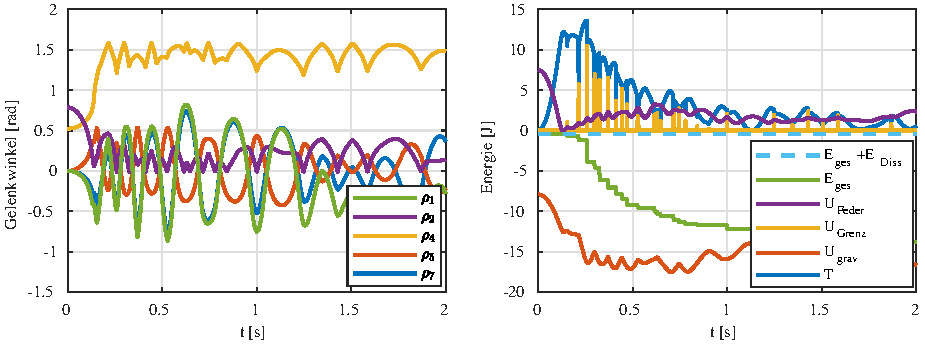
\includegraphics{figures/KAS5m5_Gelenkgrenzmodell_q_E.pdf} 
    \caption{varioations in time of a simulation to check energy consistency. Left: Minimal coordinates from (\ref{equ:mincoord}). Right: Energies (kinetic $T$, gravity $U_\mathrm{g}$, elasticity of modeled joint limits $U_\mathrm{limit}$, linear spring $U_\mathrm{s}$, total energy $E_\mathrm{total}$, Dissipated energy $E_\mathrm{Diss}$)}
    \label{fig:SimulationEnergiekonsistenz}
\end{figure*} 
%
Further, the results were compared against a SimMechanics model of the mechanism.

This simulation is extended by the use of a human upper body musculoskeletal model, coupled with an elasticity to the tool handle of the exoskeleton via the term $\bm{\tau}_{1\mathrm{ext}}$ in (\ref{equ:ForwDyn}), which is elaborated in \cite{KuehnHuSchHad2018}.
%This allows to ...


\section{Conclusions and future work}

%conclusion:
We presented a novel concept for a force assistance exoskeleton to support workers in carrying and using powertools.
In the concept of this work, the mechanism can be regarded as an academic example.
The details on the solution of the kinematic constraints of the multi-loop mechanism focus the elimination of trigonometric expressions of dependent variables to improve computational efficiency.

%Future work:
The featured approach of implementing kinematic constraints will be applied to different serial-chain industrial robots with parallel mechanisms invoking kinematic constraints, i.\,e. hybrid robots. 
The results will be compared to the classical approach using the projection of constraint forces and with non-trigonometric elimination of the constraints.

\addtolength{\textheight}{-12cm}   % This command serves to balance the column lengths
                                  % on the last page of the document manually. It shortens
                                  % the textheight of the last page by a suitable amount.
                                  % This command does not take effect until the next page
                                  % so it should come on the page before the last. Make
                                  % sure that you do not shorten the textheight too much.

%%%%%%%%%%%%%%%%%%%%%%%%%%%%%%%%%%%%%%%%%%%%%%%%%%%%%%%%%%%%%%%%%%%%%%%%%%%%%%%%



%%%%%%%%%%%%%%%%%%%%%%%%%%%%%%%%%%%%%%%%%%%%%%%%%%%%%%%%%%%%%%%%%%%%%%%%%%%%%%%%



%%%%%%%%%%%%%%%%%%%%%%%%%%%%%%%%%%%%%%%%%%%%%%%%%%%%%%%%%%%%%%%%%%%%%%%%%%%%%%%%
%\section*{APPENDIX}
%
%Appendixes should appear before the acknowledgment.


\section*{ACKNOWLEDGMENT}

...


%%%%%%%%%%%%%%%%%%%%%%%%%%%%%%%%%%%%%%%%%%%%%%%%%%%%%%%%%%%%%%%%%%%%%%%%%%%%%%%%


% BIBLIOGRAPHY
\bibliographystyle{ieeetr}
\bibliography{ref}
\end{document}
